\documentclass[autodetect-engine,dvipdfmx-if-dvi,ja=standard]{bxjsarticle}

% 二段組にするとき
% \documentclass[twocolumn,autodetect-engine,dvipdfmx-if-dvi,ja=standard]{bxjsarticle}

\usepackage{graphicx}        %図を表示するのに必要
\usepackage{color}           %jpgなどを表示するのに必要
\usepackage{amsmath,amssymb} %数学記号を出すのに必要
\usepackage{setspace}
\usepackage{eclclass}
\usepackage{cases}
\usepackage{here}
\usepackage{fancyhdr}
\usepackage{ascmac}

% 文書全体のスタイルを設定(主に余白)
\setlength{\topmargin}{-0.3in}
\setlength{\oddsidemargin}{0pt}
\setlength{\evensidemargin}{0pt}
\setlength{\textheight}{44\baselineskip}

% 行頭の字下げをしない
\parindent = 0pt

% ヘッダとフッタの設定
\lhead{電気情報工学応用実験II}
\chead{}
\rhead{5E 20番 佐藤凌雅}
\lfoot{}
\cfoot{-\thepage-} % ページ数
\rfoot{}

% 式の番号を(senction_num.num)のようにする
\makeatletter
\@addtoreset{equation}{section}
\def\theequation{\thesection.\arabic{equation}}
\makeatother

% 画像の貼り付けを簡単にする
\newcommand{\pic}[2]
{
  \begin{figure}[H]
    \begin{center}
      \includegraphics[scale=#2]{#1}
    \end{center}
  \end{figure}
}

% 単位の記述を簡単にする
\newcommand{\unit}[1]
{
  \, [\mathrm{#1}]
}
\begin{document}
% \maketitle
\pagestyle{fancy}


\section{目的}
\begin{enumerate}
\item AM変調に必要な搬送波の発振及び信号波の発振の原理を理解するとともに、AM 変調の概念を得る。
\item AM変調波の復調回路の一つである包絡線検波回路の原理を理解する。
\end{enumerate}

\section{理論}
\subsection{発振条件}
 帰還発振器は図1に示すように増幅器と帰還回路で構成される。回路が発振条件を満足しているときは、極めてわずかな衝撃、たとえば電圧印加時の過渡現象や雑音などを元にして振動増幅が次第に増大し、トランジスタの非直線に抑えられて一定の振幅に落ち着く。今、発振が成立しているとすれば帰還量Bは、増幅器の入力量$\frac{1}{A}$に等しいはずであるから式(1)が成立する。
\begin{flalign}
  A\beta &= 1
\end{flalign}

 エミッタ増幅では、入力信号と出力信号は位相が 180°異なり、Aは負の符号を持つので、Bも負の符号を持たなければならない。\\
 一方、回路のスイッチを入れたとき振動を成長させるためには、式(2)であることが必要である。
\begin{flalign}
AB>1
\end{flalign}

\subsection{CR 発振回路 (移相発振)}
 CRの帰還回路と増幅器で構成する発振回路であり能率が悪い欠点があるが、周波数は安定で変化 範囲も広くコイルを用いないので、低周波では小型にできる利点がある。\\
 図2 のように、一段のCR回路でRの端子電圧$V_o$は$V_i$に比べて$\phi$だけ位相が進む。このような 回路を何段か継続することにより 180°位相を変えることができる。図3では、回路の一段ごとの位相が進んでいくので進相型という。\\
 発振周波数fは
\begin{flalign}
  f &= \frac{1}{2 \pi \sqrt{6} C R}
\end{flalign}

増幅器の増幅度$A_V$は
\begin{flalign}
  A_V &= -29
\end{flalign}
となる。

\subsection{コレクタ同調形発振回路}
・予習課題として調査すること。


\subsection{変調回路}
 変調とは、情報源から出力される信号を、搬送波と呼ばれる正弦波またはパルス列の変化に変換することである。\\
 ある信号を$A \cos(\omega t + \phi)$で表わされる正弦波を用いて伝送しようとする場合、以下の3つの変調方法が考えられる。\\

 振幅変調: 信号の大きさに比例して振幅Aを変化させる方法\\
周波数変調: 信号の大きさに比例して角周波数(周波数)を変化させる方法\\
 位相変調: 信号の大きさに比例して位相角中を変化させる方法\\

 正弦波自体には情報は無く情報を運ぶ目的で使用されるため搬送波(Carrier) と呼ばれている。情報を持っている信号は変調信号 (Modulating Signal) と呼ぶ。搬送波が変調信号により変調され変形した波形を被変調波(Modulated Wave)という。

\subsection{コレクタ変調回路}
予習課題として調査すること。

\subsection{振幅変調のスペクトラム}
 変調信号を$A_s \cos \omega_s t$で表わされる正弦波とする場合、この信号を搬送波$A_s \cos \omega_c t$で変調したときの被変調波$f(t)$は

\begin{flalign}
f(t) &= (A_c + A_s \cos \omega_s t) \cos \omega_c t \nonumber\\
&= A_c(1 + m cos \omega_s t) cos \omega_c t
\end{flalign}

\begin{flalign}
m = \frac{A_s}{A_c}
\end{flalign}

となる\\
mを変調度(Modulation Degree)という。式(S) を変形すると
\begin{flalign}
f(t) &= A_c \cos \omega_c t + \frac{mA_c}{2} \cos(\omega_c + \omega_s)+ \frac{mA_c}{2} \cos(\omega_c - \omega_s)
\end{flalign}
になる。式(7)をスペクトルに表わすと図5のようになる。\\

\subsection{包絡線検波回路}
 被変調波は、ダイオードの整流作用により正側のみ取り出される。その後、コンデンサCと並列抵抗R($R_F$ // $R_L$)の充放電作用によって、被変調波の包絡線に近い検波出力が得られる。これを包絡線検波という。 Cを大きくすれば検波出力は包絡線に近くなるが、大きすぎると放電時定数が長くなって変調信号に追従できなくなり袈裟斬りひずみ(diagonal clipping distortion)を生じる。これを避けるためには時定数を$\frac{1}{\omega_c} << CR << \frac{1}{\omega_s}$とする。ただし、$\omega_c$は搬送波の角周波数、$\omega_s$は変調波の角周波数である。


\section{実験回路図}
\subsection{コレクタ同調形発振回路(ITF-011 上)}
\subsection{AM変調回路(ITF-011 上)}
\subsection{包絡線検波回路}

\section{使用機器}
AM変調実験装置 (ITF-011)\\
低周波発振器\\
直流電源\\
コンデンサ各種\\
包絡線検波回路(ブレッドボード)\\
オシロスコープ\\
スペクトラムアナライザ\\

\section{実験方法}
\subsection{AM変調実験装置の特性}
\subsubsection{実験装置の設定}
\begin{enumerate}
\item ITF-011 実験装置の取扱説明書に基づき、コレクタ同調形発振回路の設定を行なう。
\item 最終的に、発振周波数 100kHz が出力されていること、出力信号振幅を 4$V_{p-p}$に設定する。ここの信号は搬送波として使用する。
\end{enumerate}


\subsubsection{変調回路の入出力特性}
\begin{enumerate}
\item 搬送波と変調信号 1kHz(低周波発振器から出力)を変調回路に入力する。
\item オシロスコープに変調信号と被変調波を表示させる。
\item スペクトラムアナライザを接続する。
\item 変調度を、0.1~1.0間で三通り選択して、それぞれの波形を観測する。波形から変調度を計算する場合は、Equation(8) を使用する。
\item 各変調度におけるスペクトラムレベル [dBm] を測定し、Equation(9) より変調度の計算を行なう。
\end{enumerate}

\begin{flalign}
  m = \frac{X-Y}{X+Y}
\end{flalign}

\begin{flalign}
  m = 10 \times \frac{\mbox{上側波帯レベル} - \mbox{搬送波レベル}}{20} + 10 \times \frac{\mbox{下側波帯レベル} - \mbox{搬送波レベル}}{20}
\end{flalign}


\subsection{包絡線検波回路による信号の復調}
\begin{enumerate}
\item 被変調波を検波回路に入力する。検波回路のデフォルトは、C 無しとなっている。
\item オシロスコープに被変調波と検波波形を表示させる。コンデンサ無しの波形を観測する。
\item $\frac{1}{\omega_c} << CR << \frac{1}{\omega_s}$の条件に適したコンデンサの中から、より包絡線に近い検波波形を表示する.
\item コンデンサを接続して観測する。 4. 以下の条件を満たすコンデンサを接続して同様に観測する。
\end{enumerate}

% \begin{figure}[H]
%   \centering
%   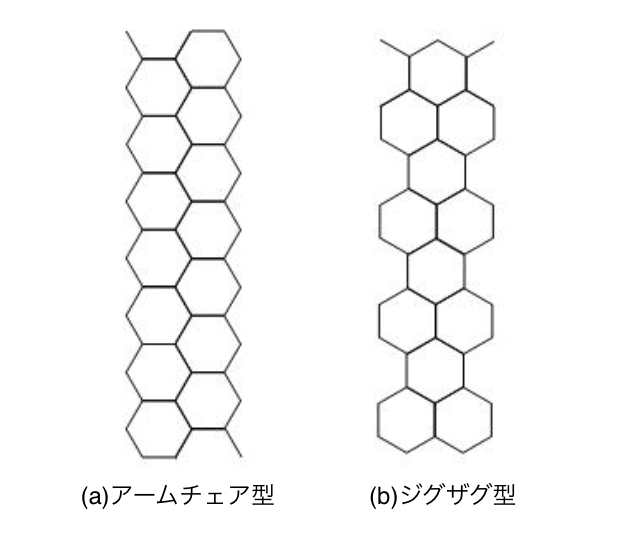
\includegraphics[height=5cm]{./data/1.png}
%   \caption{周波数変調波}
% \end{figure}


\end{document}
